\documentclass[tikz, border=10pt]{standalone}
\usepackage{tikz}
\usetikzlibrary{arrows.meta, positioning}

\begin{document}
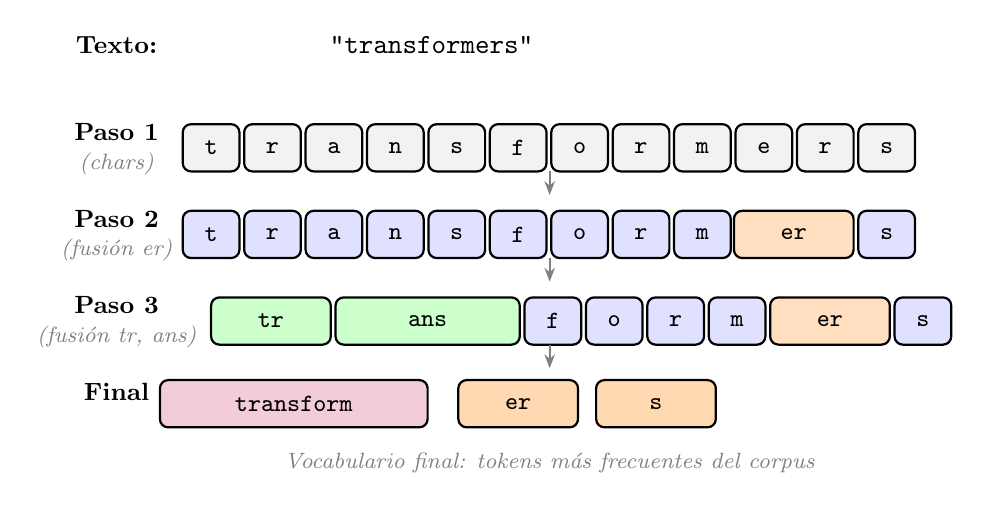
\begin{tikzpicture}[
    tok/.style={draw, rounded corners=3pt, minimum width=0.72cm, minimum height=0.6cm,
                thick, align=center, font=\ttfamily\small},
    arr/.style={-{Stealth[length=5pt]}, thick, gray},
    steplbl/.style={font=\small\bfseries},
    note/.style={font=\footnotesize\itshape, gray}
]

% ---- Step 0: raw text ----
\node[steplbl] at (-1.2, 4.0) {Texto:};
\node[font=\ttfamily] at (2.8, 4.0) {"transformers"};

% ---- Step 1: character split ----
\node[steplbl] at (-1.2, 2.9) {Paso 1};
\node[note] at (-1.2, 2.5) {(chars)};

\foreach \i/\c in {0/t,1/r,2/a,3/n,4/s,5/f,6/o,7/r,8/m,9/e,10/r,11/s} {
    \pgfmathsetmacro{\x}{\i * 0.78}
    \node[tok, fill=gray!10] at (\x, 2.7) {\c};
}

% ---- Step 2: first merges ----
\draw[arr] (4.3, 2.4) -- (4.3, 2.1);
\node[steplbl] at (-1.2, 1.8) {Paso 2};
\node[note] at (-1.2, 1.4) {(fusión er)};

\node[tok, fill=blue!12] at (0*0.78, 1.6) {t};
\node[tok, fill=blue!12] at (1*0.78, 1.6) {r};
\node[tok, fill=blue!12] at (2*0.78, 1.6) {a};
\node[tok, fill=blue!12] at (3*0.78, 1.6) {n};
\node[tok, fill=blue!12] at (4*0.78, 1.6) {s};
\node[tok, fill=blue!12] at (5*0.78, 1.6) {f};
\node[tok, fill=blue!12] at (6*0.78, 1.6) {o};
\node[tok, fill=blue!12] at (7*0.78, 1.6) {r};
\node[tok, fill=blue!12] at (8*0.78, 1.6) {m};
\node[tok, minimum width=1.52cm, fill=orange!25] at (7.40, 1.6) {er};
\node[tok, fill=blue!12] at (8.58, 1.6) {s};

% ---- Step 3: more merges ----
\draw[arr] (4.3, 1.3) -- (4.3, 1.0);
\node[steplbl] at (-1.2, 0.7) {Paso 3};
\node[note] at (-1.2, 0.3) {(fusión tr, ans)};

\node[tok, minimum width=1.52cm, fill=green!20] at (0.76, 0.5) {tr};
\node[tok, minimum width=2.34cm, fill=green!20] at (2.75, 0.5) {ans};
\node[tok, fill=blue!12] at (4.34, 0.5) {f};
\node[tok, fill=blue!12] at (5.12, 0.5) {o};
\node[tok, fill=blue!12] at (5.90, 0.5) {r};
\node[tok, fill=blue!12] at (6.68, 0.5) {m};
\node[tok, minimum width=1.52cm, fill=orange!25] at (7.86, 0.5) {er};
\node[tok, fill=blue!12] at (9.04, 0.5) {s};

% ---- Final ----
\draw[arr] (4.3, 0.2) -- (4.3, -0.1);
\node[steplbl] at (-1.2, -0.4) {Final};

\node[tok, minimum width=3.4cm, fill=purple!20] at (1.05, -0.55) {transform};
\node[tok, minimum width=1.52cm, fill=orange!30] at (3.9, -0.55) {er};
\node[tok, minimum width=1.52cm, fill=orange!30] at (5.65, -0.55) {s};

% ---- Legend ----
\node[note] at (4.3, -1.3) {Vocabulario final: tokens más frecuentes del corpus};

\end{tikzpicture}
\end{document}
